\hspace{-1.3mm}[9~v\textsuperscript{o}]
\edtext{nempe $\displaystyle MY.$}{\lemma{nempe}\Bfootnote{$\displaystyle MY.$ \textit{erg. L}}}
quae ab ipsis $\displaystyle NS$ secetur
\edtext{in $\displaystyle X$: tunc si ipsae $\displaystyle PB.$ $\displaystyle P(B).$ $\displaystyle PE$ vel
[$\displaystyle MX.$ $\displaystyle M(X).$]
$\displaystyle MY$ sint ut numeri, erunt $\displaystyle XN.$ $\displaystyle (X)(N).$ $\displaystyle YE$ ut Logarithmi seu ut spatia $\displaystyle QPBDQ.$ $\displaystyle QP(B)(D)Q.$ $\displaystyle QPEFQ$.}{\lemma{in $\displaystyle X$}\Bfootnote{%
\textit{(1)}\ . Sed jam recognoscere mihi videor errorem, in eo quod dixi illas infinitas rectas esse ut spatia illa infinita seu ut logarithmos. Erunt spa %
\textit{(2)}\ : tunc [...] $\displaystyle PE$ %
\textit{(a)}\ sint %
\textit{(b)}\ vel $\displaystyle MN.$ $\displaystyle M(N).$ [...] $\displaystyle QPEFQ$. \textit{L ändert Hrsg.}}}
\pend
\count\Bfootins=1100
\count\Cfootins=1200
\count\Afootins=1200
\pstart
Linea ergo $\displaystyle ENM$ logarithmica est.
\pend
\pstart
Ergo si $\displaystyle XN.$ $\displaystyle (X)(N).$
\edtext{$\displaystyle YE$ vel $\displaystyle MZ.$ $\displaystyle M(Z).$ $\displaystyle MP$ [sint progressionis Arithmeticae] erunt}{\lemma{$\displaystyle YE$}\Bfootnote{\textit{(1)}\ sint progressionis Arithmeticae, erunt $\displaystyle M$ \textit{(2)}\ vel $\displaystyle NZ.$ $\displaystyle (N)(Z).$ $\displaystyle EP.$ \textit{(3)}\ vel $\displaystyle MZ.$ $\displaystyle M(Z).$ $\displaystyle MP$  \textbar\ sint progressionis Arithmeticae \textit{erg. Hrsg.}\  \textbar\ erunt \textit{L}}}
$\displaystyle NZ.$ $\displaystyle (N)(Z).$ $\displaystyle EP$ progressionis Geometricae.
Sed hic jam detegitur error aliquis haud dubie admissus.
Impossibile est ut $\displaystyle NZ.$ $\displaystyle (N)(Z).$ $\displaystyle EP$ sint
\edtext{progressionis Geometricae}{\lemma{progressionis}\Bfootnote{\textit{(1)}\ Arithmeticae \textit{(2)}\ Geometricae, \textit{L}}},
quia in $\displaystyle M$ evanescerent in infinite parvam,
quod fieri non potest,
nisi infinito ab hinc intervallo seu in $\displaystyle L.$
nempe cum $\displaystyle LNE$ sit linea logarithmica,
\edtext{erunt $\displaystyle MH$ (:~$\displaystyle \, \sqcap \ PA$~:)}{\lemma{erunt}\Bfootnote{\textit{(1)}\ $\displaystyle MH \, \sqcap \, PA$ \textit{(2)}\ $\displaystyle MA$ \textit{(3)}\ $\displaystyle MH$ (:~$\displaystyle \, \sqcap \, PA$~:) \textit{L}}}
$\displaystyle NW.$ $\displaystyle (N)(W).$ \edtext{[$\displaystyle EA$]}{\lemma{$\displaystyle EP$}\Bfootnote{\textit{L ändert Hrsg.}}}
progressionis Geometricae si $\displaystyle AH.$ $\displaystyle AW.$ $\displaystyle A(W)$ sint progressionis Arithmeticae
seu \edtext{si intervalla $\displaystyle HW.$ $\displaystyle W(W).$ $\displaystyle (W)A$ sint aequalia}{\lemma{si}\Bfootnote{\textit{(1)}\ rectae $\displaystyle HW.$ $\displaystyle W(W).$ $\displaystyle (W)A$ sint aequales \textit{(2)}\ intervalla [...] aequalia. \textit{L}}}.
Accurate ergo sic loquendum est,
si $\displaystyle AP.$ $\displaystyle AB.$ \edtext{$\displaystyle A(B)$
sint}{\lemma{}\Bfootnote{$\displaystyle A(B)$  \textbar\ $\displaystyle AE$ \textit{gestr.}\ \textbar\ sint \textit{L}}}
ut numeri,
\edtext{erunt rectae $\displaystyle MP.$ $\displaystyle NB.$ $\displaystyle (N)(B)$ sive spatia $\displaystyle FEPQF.$}%
{\lemma{erunt}\Bfootnote{%
\textit{(1)}\ spatia %
\textit{(2)}\ rectae [...] spatia %
\textit{(a)}\ $\displaystyle QPEFQ.$ %
\textit{(b)}\ $\displaystyle FEPQF.$ \textit{L}}}
$\displaystyle FEBDF.$ $\displaystyle FE(B)(D)F$ ut Logarithmi.
Cum ergo rectae $\displaystyle AP.$ $\displaystyle AB.$ $\displaystyle A(B)$
\edtext{repraesentent spatia}{\lemma{repraesentent}\Bfootnote{\textit{(1)}\ numeros \textit{(2)}\ spatia \textit{L}}}
restantia et rectae $\displaystyle MP.$ $\displaystyle NB.$ $\displaystyle (N)(B)$ vel spatia dicta repraesentent tempora in\-sum\-ta.
Ideo regula erit
\edtext{talis:\textso{ Si spatia residua sint ut numeri, tempora transacta}}{\lemma{talis:}\Bfootnote{\textit{(1)}\ \textso{Si tempora transacta} \textit{(2)}\ \textso{Si spatia} [...] \textso{transacta} \textit{L}}}\textso{ erunt ut Logarithmi}.
\pend
\vspace{1.7em}
%\newpage
\pstart
\centering
[\textit{Teil 3}]
\pend
%\vspace{1em}
\count\Bfootins=1200
%\vspace{2mm}
%\pstart
%  \vspace*{1em}
%\noindent
%    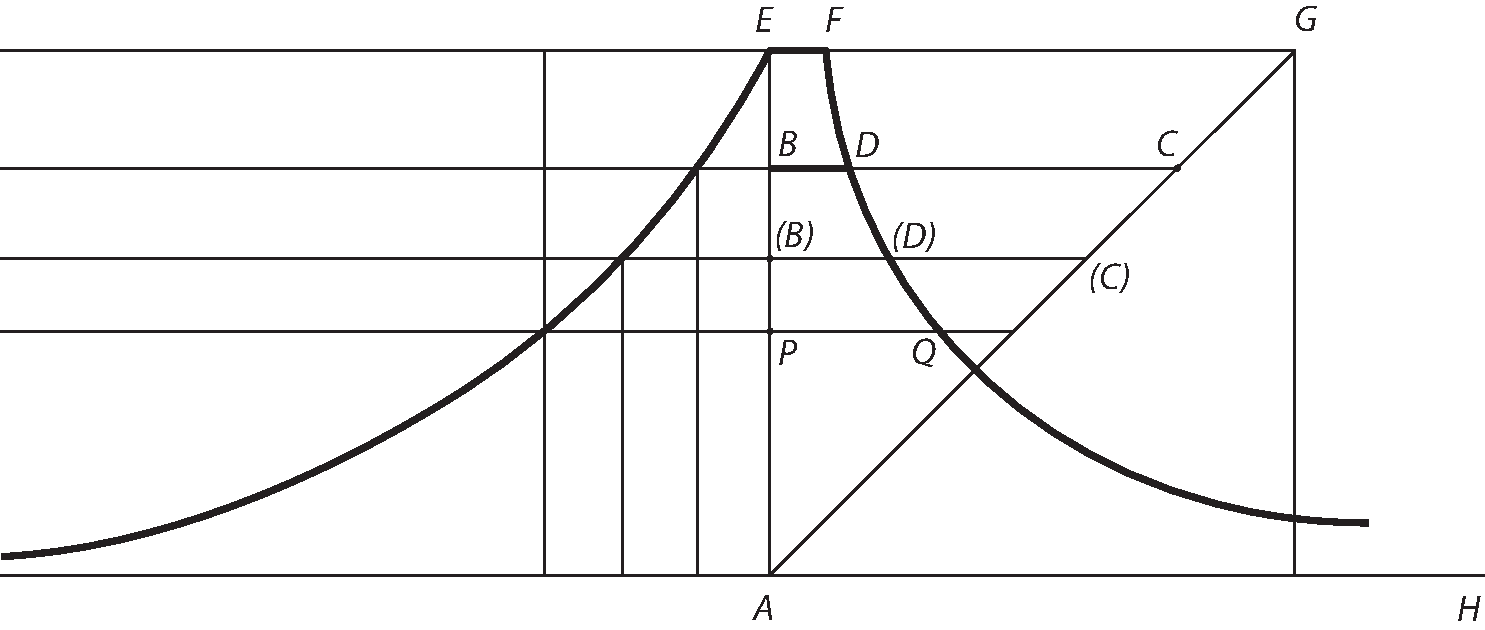
\includegraphics[trim = 0mm -3mm 0mm 0mm, clip,width=1.0\textwidth]{images/lh0350911_009v-d1.pdf}
%    \centering
%%    [\textit{Fig. 3}]\label{035,09,11_009v_Fig.3} \edtext{}{\lemma{}\killnumber\Afootnote{\textit{Am Rand unter} \textit{Fig. 3}: $\displaystyle \frac{BD}{A(B)} \sqcap \frac{AB}{(B)(D)}$\\ \\
%\hspace*{7,5mm}\textit{Darunter, ohne erkennbaren Zusammen\-hang mit dem Text:} $\displaystyle \frac{1}{1} \quad \frac{1}{2} \quad \frac{1}{3}$\vspace{-6mm}}} % \caption{Bildbeschreibung}
%   \pend
   \pstart
%\vspace*{0,5em}
\noindent
\edtext{Si mobile}{\lemma{Si}\Bfootnote{\textit{(1)}\ mobilis \textit{(2)}\ mobile \textit{L}}}
per spatium $\displaystyle EA$, ab $\displaystyle E$ versus $\displaystyle A$ ita feratur
ut in quolibet spatii puncto aequalia patiatur celeritatis decrementa\protect\index{Sachverzeichnis}{decrementum celeritatis},
donec in $\displaystyle A$ omnis ejus motus evanescat,
et prima ejus celeritas\protect\index{Sachverzeichnis}{celeritas} ponatur esse ut $\displaystyle EG$ juncta
\edtext{$\displaystyle AC$, et per}{\lemma{$\displaystyle AC$, et}\Bfootnote{\textit{(1)}\ in \textit{(2)}\ per \textit{L}}}
puncta rectae $\displaystyle EA$ spatium repraesentantis,
$\displaystyle B$ ductis $\displaystyle BC$,
applicatis Trianguli \edtext{[$\displaystyle AEG$],}{\lemma{$\displaystyle AE$}\Bfootnote{\textit{L ändert Hrsg.}}}
basi $\displaystyle EG$ parallelis,
erunt celeritates in quolibet spatii puncto $\displaystyle B$ ut applicata ei
\edtext{respondens cumque sint $\displaystyle BC$ ipsis $\displaystyle AB$ proportionales;}{\lemma{respondens}\Bfootnote{\textit{(1)}\ $\displaystyle BC.$ \textit{(2)}\ cumque [...] proportionales; \textit{L}}}
erunt\hfill celeritates\hfill residuae\hfill in\hfill quolibet\hfill puncto\hfill spatii\hfill proportionales\hfill spatio\hfill percurrendo.
\pend
\pstart
%  \vspace*{1em}
\noindent
    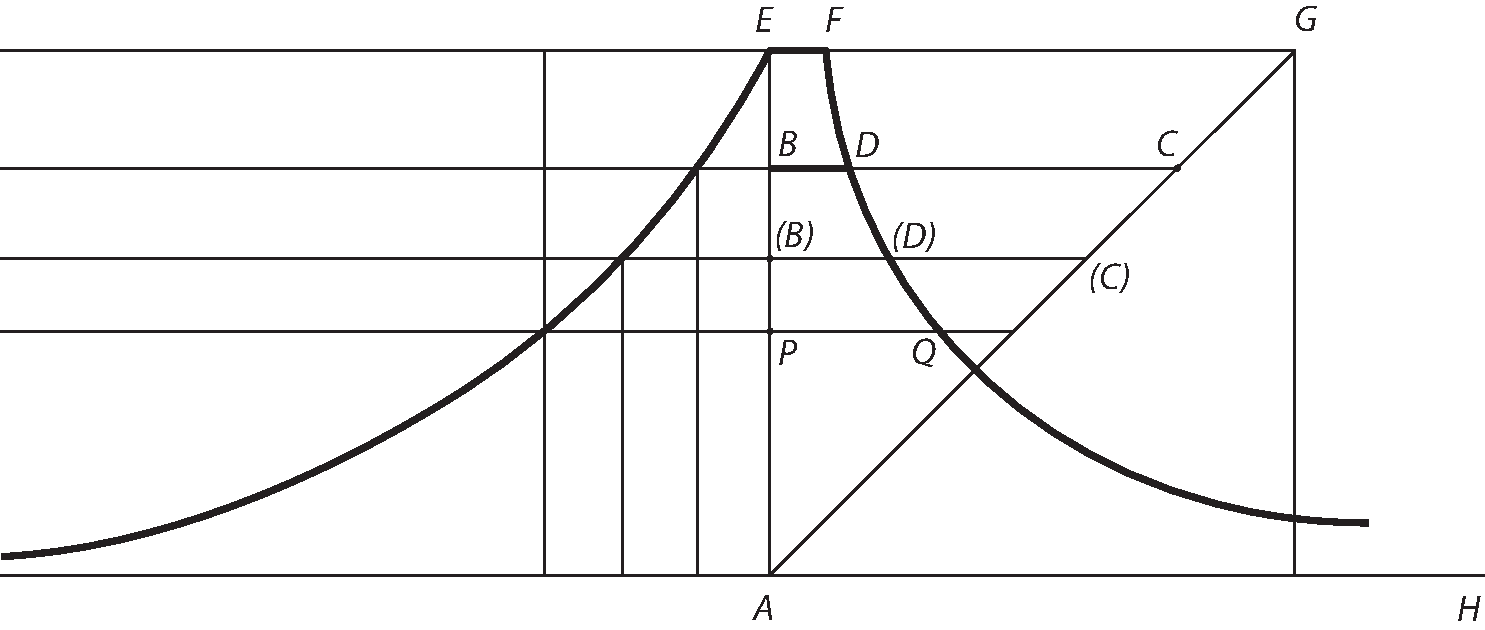
\includegraphics[trim = 0mm -3mm 0mm 0mm, clip,width=1.0\textwidth]{images/lh0350911_009v-d1.pdf}
    \centering
    [\textit{Fig. 3}]\label{035,09,11_009v_Fig.3}  % \caption{Bildbeschreibung}
   \pend
   \vspace{1.5em}
\pstart\noindent\edtext{}{\lemma{}\killnumber\Afootnote{\textit{Am Rand unter} \textit{Fig. 3}: $\displaystyle \frac{BD}{A(B)} \sqcap \frac{AB}{(B)(D)}$\\ \\
\hspace*{7,5mm}\textit{Darunter, ohne erkennbaren Zusammen\-hang mit dem Text:} $\displaystyle \frac{1}{1} \quad \frac{1}{2} \quad \frac{1}{3}$\vspace{-6mm}}}\setline{1}\edtext{Jam temporum crementa}{\lemma{Jam}\Bfootnote{\textit{(1)}\ tempora \textit{(2)}\ temporum crementa \textit{L}}}
sunt celeritatibus reciproce proportionalia[,]
celeritatibus inquam  seu  viribus\protect\index{Sachverzeichnis}{vis},
\edtext{ergo temporum crementa  sunt spatiis}{\lemma{ergo}\Bfootnote{\textit{(1)}\ tempora etiam spatiis \textit{(2)}\ temporum [...] spatiis \textit{L}}} 
residuis reciproce proportionalia quae si ponantur repraesentari per applicatas $\displaystyle BD.$ $\displaystyle (B)(D)$
vel positis $\displaystyle B(B)$ infinite parvis per areolas $\displaystyle DB(B)(D)D$,
erit curva per omnia $\displaystyle D$ transiens Hyperbola
\edtext{aequilatera}{\lemma{}\Bfootnote{aequilatera \textit{erg. L}}}
cujus centrum $\displaystyle A.$ Asymptoti ad angulos rectos $\displaystyle AE$,
\edtext{$\displaystyle AH$.\\
\hspace*{7,5mm}Positis $\displaystyle EB$, $\displaystyle B(B)$ etc. infinite parvis}{\lemma{$\displaystyle AH$.}\Bfootnote{\textit{(1)}\ Sumatur in ea punctum $\displaystyle Q$, et ducatur ad Asymptotam $\displaystyle AE$ applicata $\displaystyle PQ.$ positis  \textit{(a)}\ $\displaystyle P(B).$  \textit{(b)}\ $\displaystyle E(B).$ $\displaystyle (B)B$ etc. infinite parvis \textit{(2)}\ Positis [...] parvis, \textit{L}}},
et temporum crementis per $\displaystyle FEBDF$,
\edtext{$\displaystyle DB(B)(D)D$ areolas latitudinis infinite parvae, seu applicatas Hyperbolae repraesentatis}{\lemma{$\displaystyle DB(B)(D)D$}\Bfootnote{\textit{(1)}\ repraesentatis \textit{(2)}\ areas \textit{(3)}\ areolas  \textit{(a)}\ infinite pa  \textit{(b)}\ latitudinis [...] repraesentatis \textit{L}}}
ipsa tempora per summas eorum ac proinde per spatia Hyperbolica $\displaystyle FEBDF$, $\displaystyle FE(B)(D)F$ repraesentabuntur.
Jam sumto in recta $\displaystyle AE$ quolibet puncto% [10~r\textsuperscript{o}]
% \pend